\begin{titlepage}
   \begin{center}
       % \vspace*{1cm}

       \Large
       \textbf{Studieområdeprojekt 2019}

        \vspace{0.5cm}
        \large
        Sikkerhed bag login-formular på en hjemmeside

       \vspace{1cm}
       \large
       \textbf{Jens Tinggaard}

       \vspace{1cm}
       {\hspace{-2cm}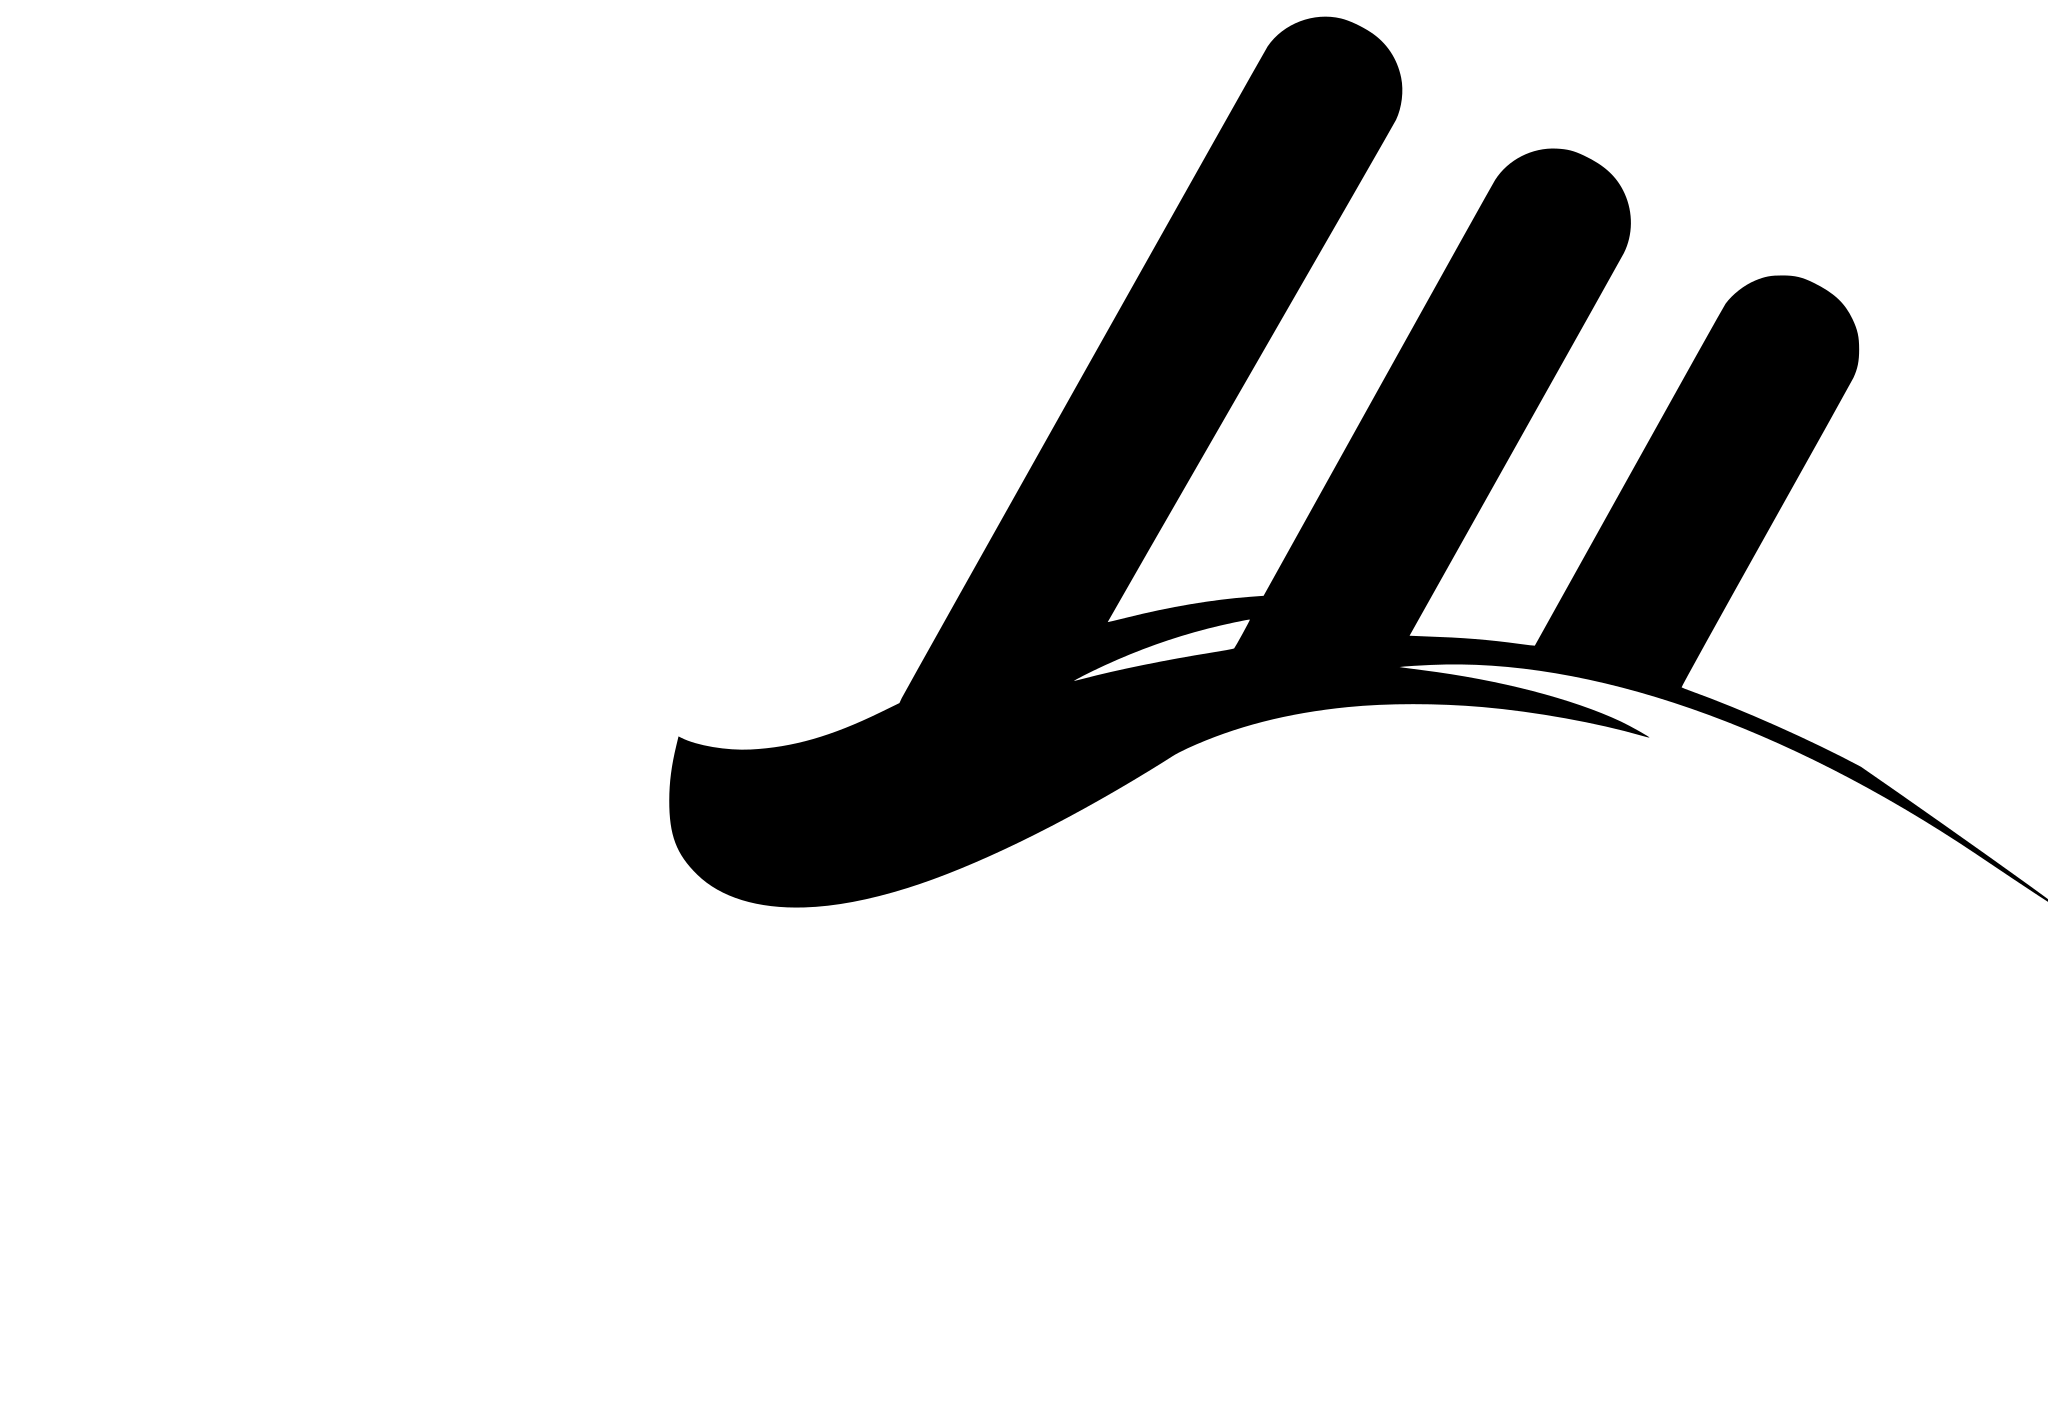
\includegraphics[width=0.4\textwidth]{img/otg_logo.png}}

       \vspace{-0.5cm}
       \begin{abstract}
           % \noindent
           I løbet af dette projekt, vil talteorien bag RSA-kryptosystemet blive gennemgået, for at kunne lave en vurdering af sikkerheden ved metoden.
           Derudover, vil metoden hashing blive sammenlignet med RSA, der vil blive udpeget fordele og ulemper ved begge metoder, samt vist hvor man bruger begge metoder på en gang.
           Slutteligt vil der være en vurdering af nødvendigheden af RSA ved logins.
           \\
           Det vil vises hvordan kryptosystemer, er nødvendige for den digitale hverdag vi lever i.
           Det vil også vises hvordan RSA både kan bruges til at kryptere data, men også bruges til online autentificering.
           Et konkreteksempel af RSA vil blive gennemgået, med forklaring af protokollerne som indgår i processen.
           Samt en forklaring af hvad man kan gøre for at øge onlinesikkerheden, både set ud fra brugerens synspunkt, men også som en systemadministrator.
       \end{abstract}

       \vfill

       Vejledere: Søren Søndergaard Eriksen \& Lena Erbs\\
       Fag: Matematik A \& Programmering B\\
       Odense Tekniske Gymnasium\\
       20. december 2019
   \end{center}
\end{titlepage}
